\documentclass[12pt]{article} % use larger type; default would be 10pt
\usepackage[czech]{babel}
\usepackage[utf8]{inputenc} % set input encoding (not needed with XeLaTeX)

%%% PAGE DIMENSIONS
\usepackage{geometry} % to change the page dimensions
% \usepackage[left=2cm,right=2cm,top=2cm,bottom=2cm]{geometry}
\geometry{a4paper}
% \geometry{margin=2in} % for example, change the margins to 2 inches all round
% \geometry{landscape} % set up the page for landscape

\usepackage{graphicx} % support the \includegraphics command and options
\usepackage{wrapfig} % support the wrapfigure section

\usepackage{hyperref} % links in \tableofcontents
\hypersetup{
	colorlinks,
	citecolor=black,
	filecolor=black,
	linkcolor=black,
	urlcolor=black
}

% \usepackage[parfill]{parskip} % Activate to begin paragraphs with an empty line rather than an indent

%%% PACKAGES
\usepackage{booktabs} % for much better looking tables
\usepackage{array} % for better arrays (eg matrices) in maths
%\usepackage{paralist} % very flexible & customisable lists (eg. enumerate/itemize, etc.)
\usepackage{verbatim} % adds environment for commenting out blocks of text & for better verbatim
\usepackage{subfig} % make it possible to include more than one captioned figure/table in a single float
% These packages are all incorporated in the memoir class to one degree or another...
\usepackage{tikz} % graphs
\usepackage{pgfplots}
\usepackage{float}

%%% HEADERS & FOOTERS
\usepackage{fancyhdr} % This should be set AFTER setting up the page geometry
\pagestyle{fancy} % options: empty , plain , fancy
\renewcommand{\headrulewidth}{0pt} % customise the layout...
\lhead{}\chead{}\rhead{}
\lfoot{}\cfoot{\thepage}\rfoot{}

%%% SECTION TITLE APPEARANCE
\usepackage{sectsty}
\allsectionsfont{\sffamily\mdseries\upshape} % (See the fntguide.pdf for font help)
% (This matches ConTeXt defaults)

%%% ToC (table of contents) APPEARANCE
\usepackage[nottoc,notlof,notlot]{tocbibind} % Put the bibliography in the ToC
\usepackage[titles,subfigure]{tocloft} % Alter the style of the Table of Contents
\renewcommand{\cftsecfont}{\rmfamily\mdseries\upshape}
\renewcommand{\cftsecpagefont}{\rmfamily\mdseries\upshape} % No bold!
\newcommand{\bigsize}{\fontsize{35pt}{20pt}\selectfont}

%%% END Article customizations

\begin{document}
\begin{titlepage}
	
\includegraphics[scale=0.7]{logo.jpg}
	\vspace*{\fill}
	\begin{center}
		\textsc{\LARGE Katedra technologií a měření}\\[0.3cm]
		\textsc{\LARGE \bigsize Fyzikální elektronika}\\[0.3cm]
		\textsc{\LARGE Měření dynamických\\charakteristik diod}\\[1cm]
		Martin Zlámal \\
		Josef Sedlák \\[1cm]
		{\small\em \ Datum měření 18. listopad 2013 } \\
		{\small\em \copyright \ Datum poslední revize \today } \\
		\LaTeX
	\end{center}
	\vspace*{\fill}
\end{titlepage}
\tableofcontents
\listoffigures
\listoftables
\newpage

\section{Schéma zapojení úlohy}
\begin{figure}[H]
\center
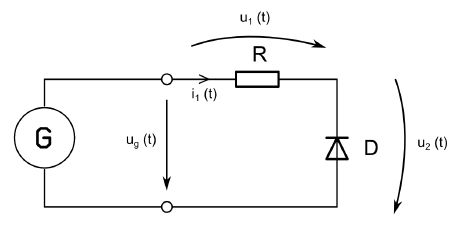
\includegraphics[scale=0.8]{schema.png}
\caption{Schéma zapojení}
\end{figure}

\section{Katalogové parametry měřených součástek}
\begin{table}[H]
\caption{Katalogové parametry měřených součástek}
\begin{tabular}{|c|c|c|}
\hline 
Typ měřené diody & Doba zotavení $t_{rr}$ & Hodnota předřadného SMD rezistoru \\ 
\hline 
1N4007G & není uváděn & $1\,k\Omega$ \\ 
\hline 
1N5062 & max. $4\,\mu s$ & $1\,k\Omega$ \\ 
\hline 
1N5625 & není uváděn & $1\,k\Omega$ \\ 
\hline 
BY448 & max. $2\,\mu s$ & $1\,k\Omega$ \\ 
\hline
BYW54 & max. $4\,\mu s$ & $1\,k\Omega$ \\ 
\hline 
\end{tabular} 
\end{table}

\section{Naměřené a vypočtené hodnoty}
\begin{table}[H]
\caption{Naměřené a vypočtené hodnoty}
\begin{tabular}{|c|c|c|c|c|c|}
\hline 
• & 1N4007G & 1N5062 & 1N5625 & BY448 & BYW54 \\ 
\hline 
$t_s\,[\mu s]$ & $2,72$ & $1,92$ & $1,88$ & $0,38$ & $3,44$ \\ 
\hline 
$t_{rr}\,[\mu s]$ & $3,96$ & $4,96$ & $7$ & $1,88$ & $8,32$ \\ 
\hline 
$t_r\,[\mu s]$ & $1,24$ & $3,04$ & $5,12$ & $1,5$ & $4,88$ \\ 
\hline 
$U_f\,[V]$ & $1,16$ & $1,24$ & $1,24$ & $1,24$ & $1,32$ \\ 
\hline 
$U_r\,[V]$ & $-2,36$ & $-2,36$ & $-2,28$ & $-2,16$ & $-2,28$ \\ 
\hline 
$I_r\,[mA]$ & $-2,36$ & $-2,36$ & $-2,28$ & $-2,16$ & $-2,28$ \\ 
\hline 
$I_f\,[mA]$ & $1,16$ & $1,24$ & $1,24$ & $1,24$ & $1,32$ \\ 
\hline 
$\tau\,[\mu s]$ & $0,413$ & $1,013$ & $1,707$ & $0,5$ & $1,627$ \\ 
\hline 
$t_s\,[\mu s]$ & $0,165$ & $0,428$ & $0,741$ & $0,227$ & $0,743$ \\ 
\hline 
$Q_s\,[nC]$ & $-6,42$ & $-4,53$ & $-4,29$ & $-0,82$ & $-7,84$ \\ 
\hline 
$f_{max}\,[kHz]$ & $126,263$ & $100,806$ & $71,429$ & $265,957$ & $60,096$ \\ 
\hline 
\end{tabular} 
\end{table}

Kde $I_r$ pro předřadný odpor $1000\,\Omega$:
\begin{equation}
I_r = \frac{U_r}{R_p} = \frac{-2,36}{1000} = -0,00236\,A
\end{equation}
$I_f$ pro předřadný odpor $1000\,\Omega$:
\begin{equation}
I_f = \frac{U_f}{R_p} = \frac{1,16}{1000} = 0,00116\,A
\end{equation}
Výpočet $\tau$:
\begin{equation}
\tau = \frac{t_r}{3} = \frac{1,24}{3} = 0,413\,\mu s
\end{equation}
Matematický výpočet $t_s$:
\begin{equation}
t_s = \tau\cdot ln\left(1+\frac{I_f}{I_r} \right) = 0,413\cdot ln\left(1+\frac{1,16}{2,36} \right) = 0,165 \,\mu s
\end{equation}
Náboj na diodě $Q_s$:
\begin{equation}
Q_s = I_r\cdot t_s = -2,36\cdot 2,72 = 6,42 \,nC
\end{equation}
Výpočet $f_{max}$:
$$t_{rr} = \frac{T}{2} \qquad ; \qquad f_{max} = \frac{1}{T}$$
\begin{equation}
f_{max} = \frac{1}{2\cdot t_{rr}} = \frac{1}{2\cdot 3,96} = 126,263\,kHz
\end{equation}

\section{Závěr}
Katalogové hodnoty doby zotavení $t_{rr}$ se vůči katalogovým hodnotám různě liší. Například diody BYW54 přesahuje dobu zotavení více než dvojnásobně, oproti tomu například dioda BY448 se svým časem $1,88\,\mu s$ se vejde do výrobcem předepsané hodnoty max. $2\,\mu s$.

Maximální spínací frekvence $f_{max}$ se liší v závislosti na typu diody. Nejpomalejší dioda je BYW54, která dokáže vzhledem k době zotavení snést $60\,kHz$. Naopak nejrychlejší dioda je BY448, která dokáže vzhledem k době zotavení snést více než $265\,kHz$.

\end{document}